\documentclass[12pt]{article}

%\documentclass[17pt]{extarticle}

%\usepackage{extsizes}
\usepackage{indentfirst}
\usepackage[utf8x]{inputenc}
\usepackage[T1]{fontenc}
\usepackage[english,lithuanian]{babel}
\usepackage{array}
\usepackage{caption}
\usepackage{makecell}
\usepackage[euler]{textgreek}
\usepackage{hyperref}

\usepackage{amsmath, amsthm, amssymb}
\usepackage{graphicx}
\usepackage{setspace}
\usepackage{verbatim}
\usepackage[left=3cm,top=2cm,right=1.5cm,bottom=2cm]{geometry}
\usepackage{floatrow}
\newfloatcommand{capbtabbox}{table}[][\FBwidth]
\usepackage{blindtext}

\onehalfspacing

\newcommand{\EE}{\mathbb{E}\,} % Mean
\newcommand{\ee}{{\mathrm e}}  % nice exponent
\newcommand{\dd}{{\mathrm d}}
\newcommand{\RR}{\mathbb{R}}

\begin{document}
\selectlanguage{lithuanian}

\begin{titlepage}
\vskip 20pt
\begin{center}

\includegraphics[scale=0.5]{MIF}
\end{center}

%%%%%%%%%%%%%%%%%%%%%%%%%%%%%%%%%%%%%%%%
% TITULINIO PUSLAPIO TEKSTAS
%%%%%%%%%%%%%%%%%%%%%%%%%%%%%%%%%%%%%%%%

\vskip 20pt
\centerline{\bf \large \textbf{VILNIAUS UNIVERSITETAS}}
\bigskip
\centerline{\large \textbf{MATEMATIKOS IR INFORMATIKOS FAKULTETAS}}
\bigskip
\centerline{\large \textbf{BIOINFORMATIKOS BAKALAURO STUDIJŲ PROGRAMA}}

\vskip 90pt
\begin{center}
    {\bf \LARGE \emph{tbx5} ir \emph{tcf21} genų įtakos regeneracijai tyrimai}
\end{center}
\begin{center}
    {\bf \Large Research of the \emph{tbx5} and \emph{tcf21} genes' functions in regeneration}
\end{center}
\vskip 20pt
\centerline{\bf \large \textbf{Kursinis darbas}}
\bigskip
\vskip 50pt

\hskip 140pt {\large Autorius: Danielė Stasiūnaitė}

\hskip 140pt{\large VU el. p.: (daniele.stasiunaite@mif.stud.vu.lt)}
\bigskip
\vskip 20pt

\hskip 140pt {\large Darbo vadovas: J. m. d. Kotryna Kvederavičiūtė}
\vskip 60pt
\vskip 60pt
\centerline{\large \textbf{Vilnius}}
\centerline{\large \textbf{2022}}
\newpage
\end{titlepage}

\selectlanguage{lithuanian}

%%%%%%%%%%%%%%%%%%%%%%%%%%%%%%%%%%%%%%%%
% TURINIO PUSLAPIS
%%%%%%%%%%%%%%%%%%%%%%%%%%%%%%%%%%%%%%%%  
\tableofcontents
\newpage

%%%%%%%%%%%%%%%%%%%%%%%%%%%%%%%%%%%%%%%%
% LIETUVIŠKOS SANTRAUKOS PUSLAPIS
%%%%%%%%%%%%%%%%%%%%%%%%%%%%%%%%%%%%%%%%  
\section*{Santrauka}
Darbo santrauka.\\

\textbf{Raktiniai žodžiai: TF, ChIP-seq, regionas?}
\newpage

%%%%%%%%%%%%%%%%%%%%%%%%%%%%%%%%%%%%%%%%
% ANGLIŠKOS SANTRAUKOS PUSLAPIS
%%%%%%%%%%%%%%%%%%%%%%%%%%%%%%%%%%%%%%%%
\section*{Summary}
Short summary of results.\\

\textbf{Keywords: TF, ChIP-seq, peak?}
\newpage

%%%%%%%%%%%%%%%%%%%%%%%%%%%%%%%%%%%%%%%%
% ĮVADO PUSLAPIS
%%%%%%%%%%%%%%%%%%%%%%%%%%%%%%%%%%%%%%%%
\section{Įvadas}
\newpage

%%%%%%%%%%%%%%%%%%%%%%%%%%%%%%%%%%%%%%%%
% DUOMENŲ APŽVALGA
%%%%%%%%%%%%%%%%%%%%%%%%%%%%%%%%%%%%%%%%
\section{Duomenų bazės ir duomenys}
\subsection{GTRD duomenų bazė}
Tyrimui naudoti duomenys atsisiųsti iš \emph{GTRD}
(Gene Transcription Regulation Database)\footnote{GTRD duomenų bazė.
Prieiga per internetą: http://gtrd.biouml.org/\#!
(žiūrėta 2022 m. birželio 6 d.).}
duomenų bazės, saugančios informaciją apie transkripcijos
sekų ir atviro chromatino regionus. Taip pat duomenų bazėje saugomi
nekartografuojamų regionų duomenys bei potencialūs žmonių bei naminių
pelių regionai, prie kurių gali jungtis transkripcijos faktoriai.

Ši duomenų bazė pasirinkta dėl sistemiškai surinktų
ChIP-seq eksperimentų, kurių metu gauti rezultatai yra unifikuotai
apdoroti ir paruošti tyrėjų meta-analizėms.

\emph{GTRD} duomenų bazėje duomenys saugomi binariniu anotacijų
formatu \emph{bigBed}, leidžiančiu atvaizduoti pasirinktą
chromosomos regioną interaktyviose genominės informacijos
vizualizavimo naršyklėse (pavyzdžiui, \emph{UCSC Genome Browser}
\footnote{\emph{UCSC Genome Browser}. Prieiga per internetą:
https://genome.ucsc.edu/ (žiūrėta 2022 m. birželio 6 d.).})
efektyviau nei tekstinis \emph{BED} formatas.

\subsection{Pasirinktų mėginių charakteristika}
Analizė atlikta, naudojantis 4 nepriklausomais eksperimentais, kuriuos
iš viso sudarė 7 biologinės replikos.
Pirmoje lentelėje pateikta informacija apie tyrimui atlikti
naudotus duomenis, surinktus iš naminės pelės (lot. \emph{Mus musculus})
ląstelių.

\begin{table}[htb]
    \newcolumntype{M}[1]{>{\centering\arraybackslash}m{#1}}
    \small
    \caption*{1 lentelė. Mėginių charakteristikos}
    %\begin{tabular}{|M{2cm}|M{3.5cm}|M{3.7cm}|M{3cm}|M{3cm}|M{0.5cm}|}
    \begin{tabular}{|c|c|c|c|c|c|c|}
    \hline
    %\thead{Sample\\ window}
    \textbf{GTRD ID} & \textbf{Ląstelių tipas} &
        \textbf{\thead{Kamienas}} & \textbf{\thead{Poveikis}} &
        \textbf{Antikūnai} & \textbf{PubMed ID}\\
    \hline
    EXP030898 & \thead{HL - 1\\ (širdies raumens)} &
                C57BL/6J & \thead{TRE\\ promotorius (2 d.)} &
                - & 21415370\\ 
    \hline
    EXP058852 & Širdies prieširdžių & C57BL/6 &
                - & \thead{Tbx5\\ (sc-17866)} & 31080136\\
    \hline
    EXP062056 & \thead{Pelių naujagimių širdies\\ fibroblastų, 
                ekspresuojančių\\ didelį kiekį T antigeno, linija} &
                CD1 & \thead{sb431542,\\ xav939} &
                \thead{anti-TBX5\\ (sc-17866x)} & 31271750\\
    \hline
    EXP058843 & \thead{MEF\\ (embrionų fibroblastai)} &
                C57BL/6 & AGHMT (2 d.) &
                \thead{anti-Tbx5\\ (sc-17866)} & 31080136\\
    \hline
    EXP058847 & \thead{MEF\\ (embrionų fibroblastai)} &
                C57BL/6 & GHMT (2 d.) &
                \thead{Tbx5\\ (sc-17866)} & 31080136\\
    \hline
    EXP058850 & \thead{MEF\\ (embrionų fibroblastai)} &
                C57BL/6 & GMT (2 d.) &
                \thead{Tbx5\\ (sc-17866)} & 31080136\\
    \hline
    EXP058856 & \thead{MEF\\ (embrionų fibroblastai)} & 
                C57BL/6 & \thead{vienas\\ faktorius (2 d.)} &
                \thead{Tbx5\\ (sc-17866)} & 31080136\\
    \hline
    \end{tabular}
\end{table}
\newpage

\subsection{Santrumpų bei pavadinimų paaiškinimai}
\begin{itemize}
    \item \textbf{HL - 1}: pelių širdies raumens ląstelės, išgautos
          iš navikinių prieširdžių kardiomiocitų linijos. Šios ląstelės
          gali betarpiškai dalintis ir spontaniškai keisti
          savo formą, vykstant širdies raumens susitraukimo/
          atsipalaidavimo procesams.
    \item \textbf{MEF}: pelių embrionų fibroblastai (angl.
          \emph{Mouse Embryonic Fibroblast}). Šiai ląstelių
          linijai būdingas ląstelių gyvybingumo apribojimas,
          reiškiantis, jog šios ląstelės greitai pasensta ir miršta.
    \item \textbf{C57BL/6}: inbrydingo (angl. \emph{inbreeding}) būdu
          išvestų naminių pelių veislė. Šios veislės pelėms
          būdingas itin tamsus kailis, padidėjęs jautrumas garsams,
          kvapams, skausmui ir žemai temperatūrai. Ši veislė
          dažnai naudojama nutukimą ir imuninę sistemą tiriančiuose
          tyrimuose.
    \item \textbf{C57BL/6J}: prie naminių pelių veislės pavadinimo
          pridėtos raidės patikslina, kurioje laboratorijoje veislės
          išvestos. 'J' raidė nurodo, kad pelių veislė išvesta Meino
          valstijoje (JAV) įsikūrusioje Džeksono laboratorijoje
          \footnote{Jackson Laboratory (RRID:SCR\_004633).}.
    \item \textbf{CD1}: autbrydingo (angl. \emph{outbreeding}) būdu
          išvestų naminių pelių veislė. Šios veislės pelėms
          būdingas baltas kailis. Taip pat CD1 pelės dažnai naudojamos
          genetiniuose, toksikologiniuose, farmakologiniuose ir
          senėjimo tyrimuose.
    \item \textbf{TRE}: tetraciklino atsako elementas (angl. 
          emph{Tetracycline Response Element}). Tai yra DNR sekos
          fragmentas. <PAPILDYTI>
    \item \textbf{sb431542}: stipriai veikianti, selektyvi cheminė
          medžiaga; transformuojančio augimo faktoriaus {\textbeta}
          (TGF-{\textbeta}) inhibitorius.
    \item \textbf{xav939}: stipriai veikianti cheminė medžiaga;
          tankirazės inhibitorius. Tankirazė slopina TERF1 baltymo,
          stabdančio telomerazės veiklą, jungimąsi prie telomerinių
          DNR sekų. <PAPILDYTI>
    \item \textbf{AGHMT}: AKT1 - serino/treonino kinazė 1; GATA4,
          HAND2, MEF2C, TBX5 - kardiogeniniai transkripcijos faktoriai.
    \item \textbf{GHMT}: GATA4, HAND2, MEF2C, TBX5.
    \item \textbf{GMT}: GATA4, MEF2C, TBX5.
    \item \textbf{sc-17866x}:
    \item \textbf{sc-17866}:
\end{itemize}


\subsection{Pasirinktų eksperimentų apžvalga}
\begin{itemize}
    \item \textbf{EXP030898}: vienas mėginys iš septyniolikos eksperimento
        metu tirtų mėginių. Eksperimente buvo siekiama patvirtinti arba
        atmesti hipotezę apie širdies stipriklių (angl. \emph{enhancer})
        identifikiavimą prie chromatino jungiantis keliems transkripcijos
        faktoriams.

        HL - 1 širdies raumens ląstelės buvo infekuotos
        su adenovirusu, ekspresuojančiu troponiną T, kuris skatina \emph{rtTA} ir
        \emph{BirA} genų ekspresiją, bei TRE promotoriumi, skatinančiu Tbx5
        transkripcijos faktoriaus geno raišką. Sąlygos taikytos 48 valandas.
    \item \textbf{EXP058852}: prieširdžių ląstelės buvo du kartus po 24
        valandas laikytos mišinyje su retrovirusais. Papildomi poveikiai nebuvo
        taikyti.
    \item \textbf{EXP062056}: eksperimente ląstelės buvo infekuotos su
        Gata4, Mef2c, ir Tbx5 transkripcijos faktorius sintetinančiais
        retrovirusais. Ląstelės augintos terpėje, kurioje buvo {Tgf\textbeta}
        inhibitoriaus sb431542, skatinančio kardiomiocitų diferenciaciją
        iš pliuripotentinių kamieninių ląstelių, ir Wnt inhibitoriaus
        xav939, stabdančio nediferencijuotų ląstelių sintezę ir
        skatinančio progenitorinių ląstelių kardiomiogenezę.
\end{itemize}

Pasirinktų duomenų rinkinyje naudoti vieno eksperimento, kuriame buvo
tirti širdies ląstelių atsinaujinimo ir diferenciacijos mechanizmai,
keturiais skirtingais poveikiais tirti mėginiai:

\begin{itemize}
    \item \textbf{EXP058843}: embrionų fibroblastai veikti AGHMT. Esant
        kardiogeniniams transkripcijos faktoriams, AKT1 skatina fibroblastų
        diferenciaciją į širdies ląsteles - kardiomiocitus.
    \item \textbf{EXP058847}: neįtraukta AKT1.
    \item \textbf{EXP058850}: į kardiogeninių transkripcijos faktorių mišinį
        neįtrauktas HAND2 transkripcijos faktorius.
    \item \textbf{EXP058856}: ląstelės veiktos tik vienu faktoriumi.
  \end{itemize}
\newpage

%%%%%%%%%%%%%%%%%%%%%%%%%%%%%%%%%%%%%%%%
% METODAI
%%%%%%%%%%%%%%%%%%%%%%%%%%%%%%%%%%%%%%%%

\section{Tyrimo metodai}
\emph{Tbx5} transkripcijos faktoriaus regionų tyrimo analizė atlikta
su R programavimo kalba\footnote{R Core Team (2022).
R: A language and environment for statistical computing. R Foundation
for Statistical Computing, Vienna, Austria. URL https://www.R-project.org/.}
(4.2.0 versija).

Tarpiniams analizės rezultatams pateikti naudotas komandinės eilutės
įrankis \emph{Scikick}\footnote{Scikick. Utility for executing collections
of computational notebooks. \\URL https://petronislab.camh.ca/pub/scikick/stable/docs/report/out\_html/introduction.html}
(0.2.0 versija), leidžiantis generuoti \emph{R Markdown (Rmd)} ataskaitas
\emph{html} formatu bei kurti struktūrizuotus puslapius, apjungiant
iš daugelio \emph{Rmd} failų gautus \emph{html} ataskaitų failus.

Žemiau esančiuose atskiruose analizės etapų skyriuose
nurodomos R bibliotekos ir papildomi komandinės eilutės įrankiai, kuriais
naudojantis pasiekti tarpiniai analizės etapų rezultatai.

\subsection{Regionų skaičiaus nustatymas mėginiuose}
\emph{Tbx5} regionų skaičius skirtinguose mėginiuose apskaičiuotas
su standartine R ilgio funkcija \emph{length()}, kuri pritaikyta
\emph{GRanges} objektui, aprašančiam genomines pozicijas bei su jomis
susijusias anotacijas. Objektas sukurtas su \emph{rtracklayer}
\footnote{M. Lawrence, R. Gentleman, V. Carey: "rtracklayer: an {R} package for
interfacing with genome browsers". Bioinformatics 25:1841-1842.}
bibliotekos funkcija \emph{import()}.
Regionų skaičių mėginiuose atvaizduojanti stulpelinė diagrama
sukurta su \emph{ggplot2}\footnote{H. Wickham. ggplot2: Elegant
Graphics for Data Analysis. Springer-Verlag New York, 2016.}
bibliotekos \emph{geom\_bar()} funkcija.

\subsection{Regionų skaičiaus nustatymas chromosomose}
Transkripcijos faktoriaus regionų skaičius skirtingose chromosomose
kiekvienam mėginiui apskaičiuotas, naudojantis standartine R
funkcija \emph{length()}, pritaikyta atskiroms chromosomoms,
kurių pozicijos aprašytos \emph{GRanges} objekte.
Kiekvieno mėginio \emph{Tbx5} transkripcijos faktoriaus pasiskirstymas
chromosomose atvaizduotas su \emph{ggplot()} ir papildoma funkcija
\emph{facet\_wrap()}, sukuriančia atskirus grafikus pagal pasirinktą
elementą - chromosomas.

\subsection{Persidengiančių regionų procentinė dalis}
Persidengiančių regionų tarp mėginių procentinė dalis nustatyta
su modifikuota \emph{Jaccard()} funkcija, apskaičiuojančia,
kiek yra sutampančių regionų tarp dviejų mėginių poros.
Naudojantis nemodifikuota funkcija, Jaccard koeficientas
apskaičiuojamas pagal išraišką:
\[ J(A, B) =  \frac{|A \cap B|}{|A \cup B|} \]

\emph{Jaccard} koeficientas gaunamas iš rinkiniams A ir B bendrų duomenų ilgio
padalinus dviejų duomenų rinkinių bendrą duomenų ilgį.

Modifikavus \emph{Jaccard} koeficiento gavimo funkciją, koeficientas
apskaičiuojamas pagal išraišką:

\[ J(A, B) = \frac{|A \cap B|}{|A|} \]

Sutampančių A ir B rinkinių duomenų ilgis padalinamas iš A rinkinio
ilgio.

\emph{Jaccard} koeficiento skaičiavimo funkcija modifikuota, nes
skaičiuojant koeficientą su standartine \emph{Jaccard} funkcija,
gaunamas itin didelis regionų sąjungos skaičius, o
persidengiančių regionų skaičius gaunamas mažas, todėl
persidengiančių regionų skaičių padalinus iš regionų sąjungos
gaunamas itin mažas koeficientas, kurio apskaičiuota procentinė
dalis neretai neviršijo 1\%.

Tam, jog būtų galima patikimiau įvertinti, kokia pirmojo mėginio
procentinė regionų dalis persidengia su antruoju mėginiu,
persidengiančių regionų skaičius padalintas iš pirmojo mėginio
regionų skaičiaus.

Gauti rezultatai atvaizduoti spalvų intensyvumo grafike (angl.
\emph{heatmap}), sukurtame su \emph{ggplot()} ir papildoma funkcija
\emph{geom\_tile()}.

\subsection{\emph{Tbx5} motyvo nustatymas}
Šiame etape genomines pozicijas aprašantys \emph{bigBed} formato
failai konvertuoti į \emph{BED} formato failus, pasinaudojus
\emph{UCSC} komandinės eilutės programa \emph{bigBedToBed}\footnote
{\emph{UCSC} komandinės eilutės programa \emph{bigBedToBed}.
Prieiga per internetą:\\ https://genome.ucsc.edu/goldenPath/help/bigBed.html.
(žiūrėta 2022 m. birželio 6 d.).}.

Sugeneruoti \emph{BED} formato failai panaudoti pikus atitinkančių
sekų iš naminės pelės genomo gavimui \emph{fasta} formatu.
Sekos iš genomo išgautos, pasinaudojus komandinės eilutės įrankio
\emph{BEDTools}\footnote{\emph{BEDTools} įrankio dokumentacija.
Prieiga per internetą:\\ 
https://bedtools.readthedocs.io/en/latest/content/bedtools-suite.html
(žiūrėta 2022 m. birželio 3 d.).}.
(2.30.0 versija) programa \emph{getfasta}\footnote{\emph{BEDTools}
įrankio programa \emph{getfasta}. Prieiga per internetą:\\
https://bedtools.readthedocs.io/en/latest/content/tools/getfasta.html
(žiūrėta 2022 m. birželio 3 d.).}.

Kiekviename mėginyje esančio \emph{Tbx5} transkripcijos faktoriaus
motyvo procentinė dalis apskaičiuota susumavus \emph{Biostrings}
\footnote{Pagès H, Aboyoun P, Gentleman R, DebRoy S (2022). \_Biostrings:
Efficient manipulation of biological strings\_. R package version
2.64.0, <https://bioconductor.org/packages/Biostrings>.}
bibliotekos funkcijos \emph{countPWM()} rezultatus bei gautą
vertę padalinus iš bendro regionų skaičiaus.

Gauta \emph{Tbx5} transkripcijos faktoriaus procentinė dalis
vizualizuota su pagrindinėmis \emph{ggplot()} ir \emph{geom\_bar()}
funkcijomis.

\subsection{Motyvų paieška \emph{de novo}}
Praturtintų sekų radimui panaudota komandinės eilutės įrankio
\emph{HOMER} \footnote{\emph{HOMER} įrankio aprašymas.
Prieiga per internetą:\\ http://homer.ucsd.edu/homer/}
(v4.11 versija) programa \emph{homer2}. Gauti
motyvai identifikuoti, pasinaudojus transkripcijos faktorių
profilių duomenų baze \emph{JASPAR}
\footnote{Castro-Mondragon JA, Riudavets-Puig R, Rauluseviciute I,
Berhanu Lemma R, Turchi L, Blanc-Mathieu R, Lucas J, Boddie P, Khan A,
Manosalva Pérez N, Fornes O, Leung TY, Aguirre A, Hammal F, Schmelter D,
Baranasic D, Ballester B, Sandelin A, Lenhard B, Vandepoele K,
Wasserman WW, Parcy F, and Mathelier A JASPAR 2022: the 9th release of
the open-access database of transcription factor binding profiles Nucleic
Acids Res. 2022 Jan 7;50(D1):D165-D173.; doi: 10.1093/nar/gkab1113}.

\subsection{Sekų praturtinimo analizė}
Pildoma...

\newpage

%%%%%%%%%%%%%%%%%%%%%%%%%%%%%%%%%%%%%%%%
% GAUTŲ REZULTATŲ APŽVALGA
%%%%%%%%%%%%%%%%%%%%%%%%%%%%%%%%%%%%%%%%

%%%%%%%%%%%%%%%%%%%%%%%%%%%%%%%%%%%%%%%%
% REGIONŲ SKAIČIUS MĖGINIUOSE
%%%%%%%%%%%%%%%%%%%%%%%%%%%%%%%%%%%%%%%%
\section{Rezultatai ir jų aptarimas}
\subsection{Regionų skaičiaus skirtumai tarp mėginių}
Pirmajame analizės etape kiekviename mėginyje nustatytas bendras
regionų skaičius pavaizduotas pirmame paveiksle.

\begin{figure}[htb]
    \begin{center}
        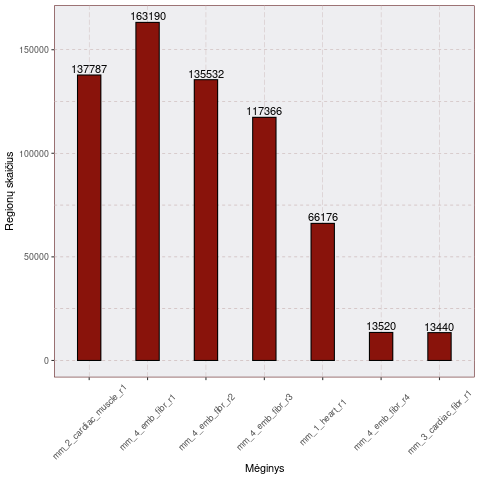
\includegraphics[width=0.7\linewidth]{Figures/total_peak_counts.png}
        \caption*{1 pav. Regionų skaičių kiekviename mėginyje
        vaizduojanti stulpelinė diagrama}
    \end{center}
\end{figure}

Remiantis diagrama didžiausias \emph{tbx5} transkripcijos faktoriaus
regionų skaičius nustatytas eksperimento \emph{(mm\_4\_emb\_fibr\_r1)}
biologinėje replikoje, kurioje pelių embrionų fibroblastų ląstelės
dvi dienas veiktos AGHMT faktoriais.
Šį rezultatą palyginus su kitomis biologinėmis replikomis, kuriose
tirtas tas pats pelių embrionų fibroblastų ląstelių kamienas, tačiau
ląstelės veiktos tik kai kuriais faktoriais, pastebimas gradualus
\emph{tbx5} transkripcijos faktoriaus regionų skaičiaus mažėjimas
diagramoje \emph{mm\_4\_emb\_fibr\_r2}, \emph{mm\_4\_emb\_fibr\_r3} ir
\emph{mm\_4\_emb\_fibr\_r4} pavaizduotuose stulpeliuose.

Mėginyje, kuriame embrionų fibroblastai veikti tik vienu faktoriumi,
\emph{tbx5} transkripcijos faktoriaus regionų nustatyta nedaug -
13520.

Mažiausiai regionų nustatyta mėginyje, kuriame tirta pelių
naujagimių širdies fibroblastų, ekspresuojančių T antigeną
ir paveiktų inhibitoriais: sb431542 ir xav939.
Nepaisant to, kad abu inhibitoriai skatina širdies ląstelių
diferenciaciją\footnote{Drowley L, Koonce C, Peel S, et al.
Human Induced Pluripotent Stem Cell-Derived Cardiac Progenitor
Cells in Phenotypic Screening: A Transforming Growth Factor-β
Type 1 Receptor Kinase Inhibitor Induces Efficient Cardiac
Differentiation. Stem Cells Transl Med. 2016;5(2):164-174.
doi:10.5966/sctm.2015-0114}, itin mažas transkripcijos
faktoriaus regionų skaičius rodo, kad papildomas veikimas
inhibitoriais daro mažą įtaką transkripcijos faktoriaus
jungimuisi prie DNR sekų.

\newpage

%%%%%%%%%%%%%%%%%%%%%%%%%%%%%%%%%%%%%%%%%%%%%
% REGIONŲ SKAIČIUS ATSKIROSE CHROMOSOMOSE
%%%%%%%%%%%%%%%%%%%%%%%%%%%%%%%%%%%%%%%%%%%%%
\subsection{Regionų pasiskirstymas chromosomose}
Nustačius \emph{tbx5} transkripcijos faktoriaus regionų
pasiskirstymą eksperimentų mėginiuose, kitame analizės etape
patikrinta, kaip faktoriaus regionai pasiskirstę atskirose
chromosomose.

Vaizduojamuose grafikuose didžiausias regionų skaičius nustatomas
pirmoje, antroje ir penktoje chromosomose. Naminės pelės pirmoji
chromosoma yra pati didžiausia, turinti 195 milijonų bazių porų,
antroji chromosoma sudaryta iš 182 megabazių, penktoji chromosoma -
152 milijonų bazių porų, todėl didesnis regionų skaičius šiose
chromosomose nėra neįprastas reiškinys. Kitose chromosomose regionų
skaičius yra mažesnis. Ypač mažas regionų skaičius nustatytas
devynioliktoje (61 Mbp), X (169 Mbp) ir Y (91 Mbp) chromosomose.

\begin{figure}[htb]
    \begin{center}
        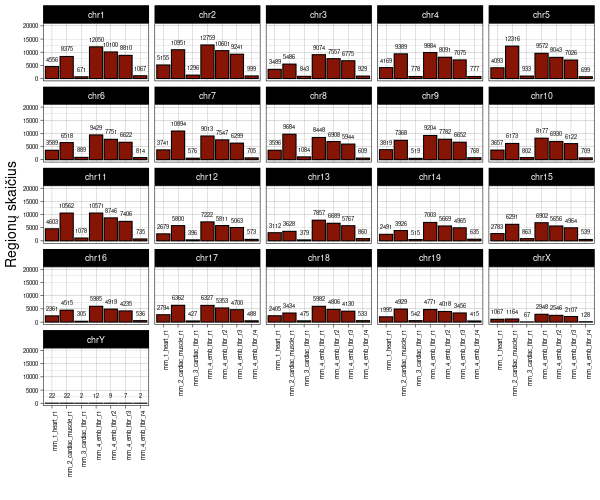
\includegraphics[width=0.8\linewidth]{Figures/peak_counts_by_chromosome.png}
        \caption*{2 pav. Regionų pasiskirstymas chromosomose}
    \end{center}
\end{figure}

Biologinių replikų mėginiuose didžiausias regionų skaičius
nustatytas antroje chromosomoje. Taip pat grafikuose išsiskiria
kontrolinis HL - 1 širdies ląstelių mėginys, kuriame didžiausias
regionų skaičius nustatytas penktojoje chromosomoje.

Remiantis pavaizduotomis regionų skaičiaus pasiskirstymo
chromosomose stulpelinėmis diagramomis, itin išsiskiriantis
atrankumas chromosomų atžvilgiu nenustatytas, todėl galima
teigti, jog šiame analizės etape duomenų problematiškumas
nepastebimas arba jo nėra.

\newpage

%%%%%%%%%%%%%%%%%%%%%%%%%%%%%%%%%%%%%%%%%%%%
% TARP MĖGINIŲ PERSIDENGIANTYS REGIONAI
%%%%%%%%%%%%%%%%%%%%%%%%%%%%%%%%%%%%%%%%%%%%
\subsection{Tarp mėginių persidengiantys regionai}
Dažnai siekiant nustatyti mėginių panašumą, yra tiriama, kokia
mėginių duomenų dalis persidengia.

\begin{figure}[htb]
    \begin{center}
        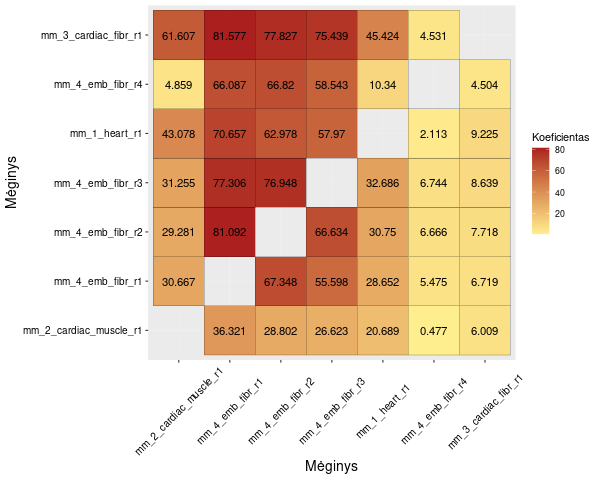
\includegraphics[width=0.8\linewidth]{Figures/peak_overlaps_between_samples.png}
        \caption*{3 pav. Persidengiančių regionų procentinės dalies vaizdavimas}
    \end{center}
\end{figure}

Remiantis pavaizduoto spalvų intensyvumo grafiko duomenimis,
didžiausi persidengiančių regionų procentai nustatyti tarp
šių mėginių:
\begin{itemize}
    \item \textbf{81.577 \%} - tarp mėginio, kuriame buvo tiriamos širdies
            fibroblastų ląstelės, ekspresuojančios T antigeną, ir mėginio,
            kuriame tirti embrionų fibroblastai, veikiant AGHMT.
    \item \textbf{81.092 \%} - tarp mėginio, kuriame tirti embrionų
            fibroblastai ir mėginio, kuriame nebuvo AKT1.
    \item \textbf{77.827 \%} - tarp mėginio su T antigeną ekspresuojančiomis
            širdies fibroblastų ląstelėmis ir mėginio, kuriame nebuvo AKT1.
    \item \textbf{76.948 \%} - tarp mėginio, kuriame nebuvo HAND2
            faktoriaus, ir mėginio, kuriame nebuvo AKT1.
    \item \textbf{75.439 \%} - tarp mėginio su T antigeną ekspresuojančiomis
            širdies fibroblastų ląstelėmis ir tarp mėginio, kuriame nebuvo HAND2
            faktoriaus.
  \end{itemize}

%%%%%%%%%%%%%%%%%%%%%%%%%%%%%%%%%%%%
% TBX5 MOTYVO NUSTATYMAS
%%%%%%%%%%%%%%%%%%%%%%%%%%%%%%%%%%%%
\subsection{\emph{Tbx5} motyvo pasiskirstymas mėginiuose}
Ketvirtajame grafike vaizduojama, kiek \emph{Tbx5}
motyvo atitikimų nustatyta skirtinguose mėginiuose.

\begin{figure}[htb]
    \begin{center}
        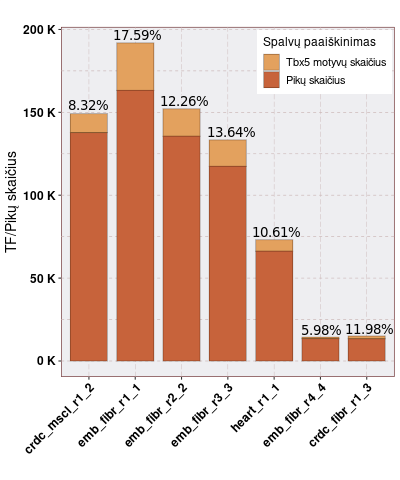
\includegraphics[width=0.7\linewidth]{Figures/tf_hit_percentage.png}
        \caption*{4 pav. \emph{Tbx5} motyvų atitikimų skaičiaus palyginimo
                  sudėtinė diagrama}
    \end{center}
\end{figure}

Antroje lentelėje (2 lentelė) nurodoma, kokią procentinę dalį
tarp visų mėginių regionų sudaro Tbx5 motyvai.

\begin{table}[htb]
    \newcolumntype{M}[1]{>{\centering\arraybackslash}m{#1}}
    \small
    \caption*{2 lentelė. Mėginių charakteristikos}
    \begin{tabular}{|c|c|}
    \hline
    \textbf{Mėginys} & \textbf{Procentinė dalis}\\
    \hline
        \emph{mm\_2\_cardiac\_muscle\_r1} & 8.32\%\\ 
    \hline
        \emph{mm\_4\_emb\_fibr\_r1} & 17.59\%\\
    \hline
        \emph{mm\_4\_emb\_fibr\_r2} & 12.26\%\\
    \hline
        \emph{mm\_4\_emb\_fibr\_r3} & 13.64\%\\
    \hline
        \emph{mm\_1\_heart\_r1} & 10.61\%\\
    \hline
        \emph{mm\_4\_emb\_fibr\_r4} & 5.98\%\\
    \hline
        \emph{mm\_3\_cardiac\_fibr\_r1} & 11.98\%\\
    \hline
    \end{tabular}
\end{table}

\newpage

\subsection{\emph{De novo} nustatytų motyvų biologinės funkcijos}
Pildoma...

\newpage

%%%%%%%%%%%%%%%%%%%%%%%%%%%%%%%%%%%%%%%%
% LITERATŪROS ŠALTINIAI
%%%%%%%%%%%%%%%%%%%%%%%%%%%%%%%%%%%%%%%%

\bibliographystyle{plain}
\begin{thebibliography}{99}
% \emph{bigBedToBed} aprašymas: https://genome.ucsc.edu/goldenPath/help/bigBed.html
% \emph{BEDTools} paketo dokumentacija: https://bedtools.readthedocs.io/en/latest/content/bedtools-suite.html
% \emph{getfasta} funkcijos dokumentacija: https://bedtools.readthedocs.io/en/latest/content/tools/getfasta.html
\end{thebibliography}
\newpage

%%%%%%%%%%%%%%%%%%%%%%%%%%%%%%%%%%%%%%%%
% PRIEDAI
%%%%%%%%%%%%%%%%%%%%%%%%%%%%%%%%%%%%%%%%

\section{Priedas}

\end{document}
